\documentclass[main.tex,fontsize=8pt,paper=a4,paper=portrait,DIV=calc,]{scrartcl}
% Document
\usepackage[T1]{fontenc}
\usepackage[utf8]{inputenc}
\usepackage[dvipsnames]{xcolor}
\usepackage[nswissgerman,english]{babel} 
\usepackage{hyperref}
\renewcommand{\familydefault}{\sfdefault}

% Format
\usepackage[top=5mm,bottom=5mm,left=5mm,right=5mm]{geometry}
%\setlength{\headheight}{\baselineskip}
%\setlength{\headsep}{0mm}

%\usepackage{scrlayer-scrpage}
%\clearpairofpagestyles
%\chead{{\bfseries\TITLE, \AUTHOR, \pagename~\thepage}}

%\addtokomafont{pagehead}{\upshape}

\usepackage{multicol}
\setlength{\columnsep}{2mm}
\setlength{\columnseprule}{0.1pt}

% Math
\usepackage{amsmath}
\usepackage{amssymb}
\usepackage{amsfonts}

% Code
\usepackage{fancyvrb, etoolbox, listings, xcolor}
%\usemintedstyle{bw}

%\newminted[shell]{bash}{
%fontsize=\footnotesize,
%fontfamily=tt,
%breaklines=true,
%frame=single,
%framerule=0.1pt,
%framesep=2mm,
%tabsize=2
%}
%\newminted{css}{
%breaklines=true,
%tabsize=4,
%autogobble=true,
%escapeinside=||,
%stripall=true,
%stripnl=true,
%}

    \definecolor{lightgray}{rgb}{0.95, 0.95, 0.95}
    \definecolor{darkgray}{rgb}{0.4, 0.4, 0.4}
    \definecolor{purple}{rgb}{0.65, 0.12, 0.82}
    \definecolor{ocherCode}{rgb}{1, 0.5, 0} % #FF7F00 -> rgb(239, 169, 0)
    \definecolor{blueCode}{rgb}{0, 0, 0.93} % #0000EE -> rgb(0, 0, 238)
    \definecolor{greenCode}{rgb}{0, 0.6, 0} % #009900 -> rgb(0, 153, 0)
    \definecolor{teal}{rgb}{0.0, 0.5, 0.5}

\lstdefinestyle{code}{
    identifierstyle=\color{black},
    keywordstyle=\color{blue}\bfseries\small,
    ndkeywordstyle=\color{greenCode}\bfseries\small,
    stringstyle=\color{ocherCode}\ttfamily\small,
    commentstyle=\color{teal}\ttfamily\textit\small,
    basicstyle=\ttfamily\small,
    breakatwhitespace=false,         
    breaklines=true,                 
    captionpos=b,                    
    keepspaces=true,                 
    showspaces=false,                
    showstringspaces=false,
    showtabs=false,                  
    tabsize=2,
    belowskip=-5pt
}



% Images
\usepackage{graphicx}
\newcommand{\pic}{\includegraphics[scale=0.3]}
\graphicspath{{Screenshots/}{../Screenshots}}
\makeatletter
\def\pictext#1#2{%
    \@ifnextchar[{%
    \pictext@iiiii{#1}{#2}%
    }{%
      \pictext@iiiii{#1}{#2}[0.5,0.4,0.3]% Default is 5
    }%
}
\def\pictext@iiiii#1#2[#3,#4,#5]{\begin{minipage}{#3\textwidth}\includegraphics[scale=#4]{#1}\end{minipage}\begin{minipage}{#5\textwidth}#2\end{minipage}}
\def\minipg#1#2{%
    \@ifnextchar[{%
    \minipg@iiii{#1}{#2}%
    }{%
      \minipg@iiii{#1}{#2}[0.3,0.6]% Default is 5
    }%
}
\def\minipg@iiii#1#2[#3,#4]{\vspace{0.8mm}\begin{minipage}{#3\textwidth}#1\end{minipage}\begin{minipage}{#4\textwidth}#2\end{minipage}{\vspace{0.8mm}}}
\makeatother

%\newenvironment{minty}[2]% environment name
%{% begin code
%  \begin{minipage}{#1}
%  \begin{minted}{#2}
%}%
%{% end code
%  \end{minted}
%  \end{minipage}
%  \end{minty}\ignorespacesafterend
%} 

% Smaller Lists
\usepackage{enumitem}
\setlist[itemize,enumerate]{leftmargin=3mm, labelindent=0mm, labelwidth=1mm, labelsep=1mm, nosep}
\setlist[description]{leftmargin=0mm, nosep}
\setlength{\parindent}{0cm}

% Smaller Titles
\usepackage[explicit]{titlesec}

%% Color Boxes
\newcommand{\sectioncolor}[1]{\colorbox{black!60}{\parbox{0.97\linewidth}{\color{white}#1}}}
\newcommand{\subsectioncolor}[1]{\colorbox{black!50}{\parbox{0.97\linewidth}{\color{white}#1}}}
\newcommand{\subsubsectioncolor}[1]{\colorbox{black!40}{\parbox{0.97\linewidth}{\color{white}#1}}}
\newcommand{\paragraphcolor}[1]{\colorbox{black!30}{\parbox{0.97\linewidth}{\color{white}#1}}}
\newcommand{\subparagraphcolor}[1]{\colorbox{black!20}{\parbox{0.97\linewidth}{\color{white}#1}}}

%% Title Format
\titleformat{\section}{\vspace{0.3mm}\bfseries}{}{0mm}{\sectioncolor{\thesection~#1}}[{\vspace{0.3mm}}]
\titleformat{\subsection}{\vspace{0.3mm}\bfseries}{}{0mm}{\subsectioncolor{\thesubsection~#1}}[{\vspace{0.3mm}}]
\titleformat{\subsubsection}{\vspace{0.3mm}\bfseries}{}{0mm}{\subsubsectioncolor{\thesubsubsection~#1}}[{\vspace{0.3mm}}]
\titleformat{\paragraph}{\vspace{0.3mm}\bfseries}{}{0mm}{\paragraphcolor{\theparagraph~#1}}[{\vspace{0.3mm}}]
\titleformat{\subparagraph}{\vspace{0.3mm}\bfseries}{}{0mm}{\subparagraphcolor{\thesubparagraph~#1}}[{\vspace{0.3mm}}]

%% Title Spacing
\titlespacing{\section}{0mm}{0mm}{0mm}
\titlespacing{\subsection}{0mm}{0mm}{0mm}
\titlespacing{\subsubsection}{0mm}{0mm}{0mm}
\titlespacing{\paragraph}{0mm}{0mm}{0mm}
\titlespacing{\subparagraph}{0mm}{0mm}{0mm}

%% format cells
\usepackage[document]{ragged2e}
\usepackage{array, makecell}
\renewcommand{\arraystretch}{2}
\newcommand{\mc}{\makecell[{{m{1\linewidth}}}]}



\title{Physics}
\author{Fabio Lenherr}

\begin{document}

\tableofcontents

\section{Terms and Definitions}

\begin{multicols*}{2}

\section{General Rules}
All physical rules are universal, this means there is no space in the universe where these rules do not apply.\newline
In other words, shit like equestria is sadly not possible according to physics, what a surprise!

\section{Shape Formulas}
\subsection{Circle}
\minipg{
\, \newline
\large \textcolor{purple}{\( C = \pi * 2 r \)}\newline
\, \newline
\large \textcolor{purple}{\( A = \pi * r^2 \)}\newline
\, \newline
\normalsize 
Legend: \newline
\begin{itemize}
\item r = radius
\item C = circumference
\item A = area 
\end{itemize}
}{
  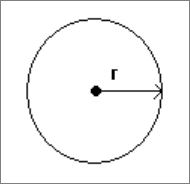
\includegraphics[scale=0.4]{2023_01_02_03_55_56.png}
}[0.25,0.25]

\subsection{Triangle}
\minipg{
\, \newline
\large \textcolor{purple}{\( C = a + b + c \)}\newline
\, \newline
\large \textcolor{purple}{\( A = \dfrac{1}{2} * b * h \)}\newline
\, \newline
\large \textcolor{purple}{\( c = \sqrt{a^2 + b^2} \)}\newline
(if 90 degree angle triangle) -> otherwise use trigonometry (SohCahToa)\newline
\normalsize 
Legend: \newline
\begin{itemize}
\item C = circumference
\item a,b,c = all sides of triangle\newline
b bottom side with 90 degree angle to height
\item h = height 
\item A = area
\end{itemize}
}{
  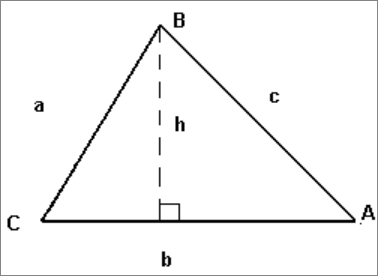
\includegraphics[scale=0.3]{2023_01_02_03_56_02.png}
}[0.25,0.25]

\subsubsection{sin/cos and tan} 
\, \newline
\large \textcolor{purple}{\( tan(\alpha) = \dfrac{sin(\alpha)}{cos(\alpha)} \)}\newline
\, \newline
\normalsize 

\subsection{Parallelogram}
\minipg{
\, \newline
\large \textcolor{purple}{\( A = b * h \)}\newline
\, \newline
\normalsize 
Legend: \newline
\begin{itemize}
\item A = area
\item b = bottom line
\item h = height 
\end{itemize} 
}{
  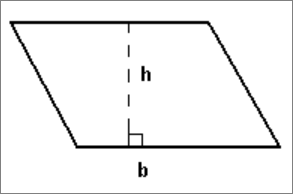
\includegraphics[scale=0.4]{2023_01_02_03_56_07.png}
}[0.25,0.25]

\subsection{Trapezoid}
\minipg{
\, \newline
\large \textcolor{purple}{\( A = \dfrac{1}{2} * (a + b) * h \)}\newline
\, \newline
\normalsize 
Legend: \newline
\begin{itemize}
\item A = area
\item a = top line
\item b = bottom line 
\item h = height
\end{itemize} 
}{
  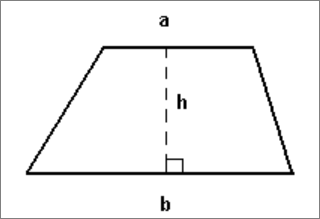
\includegraphics[scale=0.4]{2023_01_02_03_56_15.png}
}[0.25,0.25]

\subsection{Circular Sector}
\minipg{
\, \newline
\large \textcolor{purple}{\( A = \dfrac{1}{2} * r^2 * \alpha \)}\newline
\, \newline
\large \textcolor{purple}{\( s = r * \alpha \)}
\, \newline
\normalsize 
Legend: \newline
\begin{itemize}
\item s = Arclength -> length of sector
\item \(\alpha\) = angle 
\item r = radius 
\item A = area 
\end{itemize} 
}{
  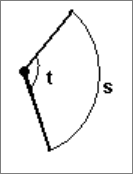
\includegraphics[scale=0.4]{2023_01_02_03_56_19.png}
}[0.25,0.25]

\subsection{Sphere}
\minipg{
\, \newline
\large \textcolor{purple}{\( V = \dfrac{4}{3} * \pi * r^3 \)}\newline
\, \newline
\large \textcolor{purple}{\( SA = 4 * \pi * r^2 \)}\newline
\, \newline
\normalsize 
Legend: \newline
\begin{itemize}
\item V = volume
\item SA = surface area
\item r = radius 
\end{itemize} 
}{
  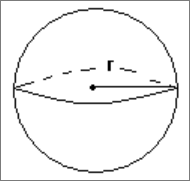
\includegraphics[scale=0.4]{2023_01_02_03_56_24.png}
}[0.25,0.25]

\subsection{Cylinder}
\minipg{
\, \newline
\large \textcolor{purple}{\( V = \pi * r^2 * h \)}\newline
\, \newline
\large \textcolor{purple}{\( SA = 2 * \pi * r * h + 2 * \pi * r^2 \)}
\, \newline
\normalsize 
Legend: \newline
\begin{itemize}
\item V = volume
\item SA = surface area
\item r = radius 
\item h = height of cylinder
\end{itemize} 
}{
  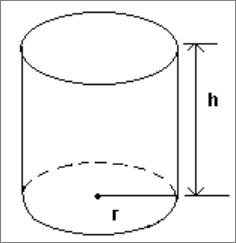
\includegraphics[scale=0.4]{2023_01_02_03_56_27.png}
}[0.25,0.25]

\subsection{Circular Cone}
\minipg{
\, \newline
\large \textcolor{purple}{\( V = \dfrac{1}{3} * \pi * r^2 * h \)}\newline
\, \newline
\large \textcolor{purple}{\( SA = \pi * r * \sqrt{r^2 + h^2} \)}\newline
\, \newline
\normalsize 
Legend: \newline
\begin{itemize}
\item V = volume
\item SA = surface area
\item r = radius 
\item h = height
\end{itemize} 
}{
  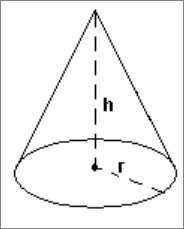
\includegraphics[scale=0.4]{2023_01_02_03_56_30.png}
}[0.25,0.25]

\section{Vectors}
\textbf{Notation} \( \vec{A} = \begin{bmatrix}x_{1} \\ x_{2} \end{bmatrix} \) OR \(\vec{A} = (x1 | x2)\)\newline
As you have learned in vocational school, use the first for vectors, the second for points.\newline

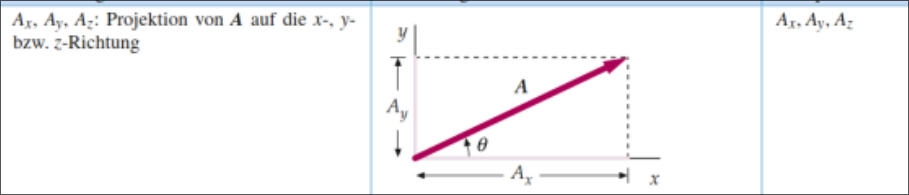
\includegraphics[scale=0.3]{2022-09-23-10:41:26.png}
{A vector is nothing but a projection in the X,Y,Z planes \newline 
It has both a direction and a value \newline
This value is usually modified by a scalar aka a factor. Then the vector can be something more universal \newline
We call this universal vector a unit vector. A directional vector with the value 1.}[0.3,0.3,0.2]\newline
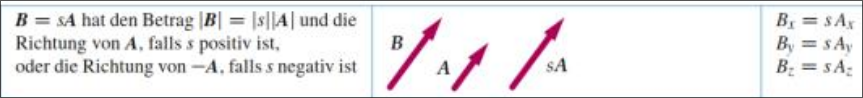
\includegraphics[scale=0.3]{2022-09-23-10:41:32.png}
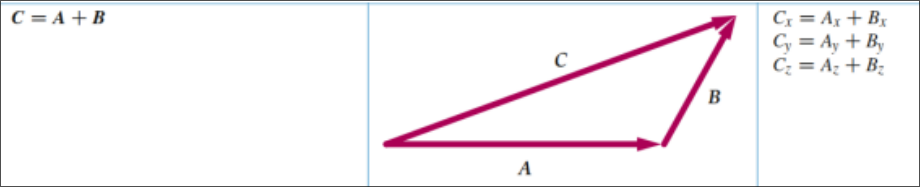
\includegraphics[scale=0.3]{2022-09-23-10:41:37.png}\newline
If the direction and the value is the same, then there is nothing that differentiates this vector from another.\newline
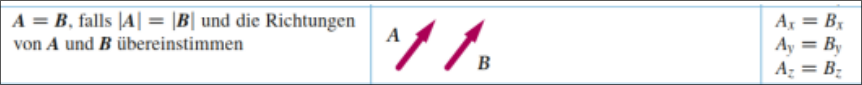
\includegraphics[scale=0.3]{2022-09-23-10:41:44.png}\newline
A vector is identical if both the value and the direction is the same.\newline
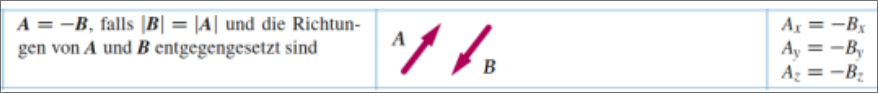
\includegraphics[scale=0.3]{2022-09-23-10:41:48.png}\newline 
Similar, if the value is identical but the direction is negated, then you have the inverse vector.\newline
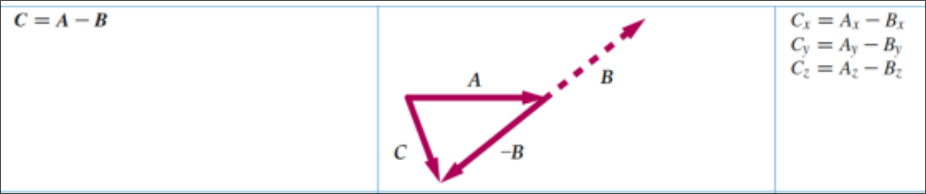
\includegraphics[scale=0.3]{2022-09-23-10:41:53.png}\newline 
simple vector math \newline
\subsection{Dotproduct}
\Large{\textbf{\textcolor{red}{\( \vec{a} * \vec{b} = |\vec{a}| * |\vec{b}| * cos(\alpha) \)}}}\newline
\normalsize This returns a scalar, aka a number that you can use.\newline
This will return 0 when used in a right angle as \(cos(90)\) is 0!\\
\subsection{Crossproduct}
\Large{\textbf{\textcolor{red}{\( \vec{a} \text{ x } \vec{b} = |\vec{a}| * |\vec{b}| * sin(\alpha) * n \)}}}\newline
\normalsize This is usually used to get the unit vector of the resulting vector.\newline
\(\alpha\) is the angle between the vector \(\vec{a}\) and \(\vec{b}\)\newline
\emph{\textcolor{teal}{For more information and proof, check the dedicated vector Document from vocational school.}}\\

\subsection{SohCahToa}
\minipg{
\, \newline
\large \textcolor{purple}{\( sine(\alpha) = \dfrac{\text{opposite}}{\text{hypotenus}} \)}\newline
\large \textcolor{purple}{\( cos(\alpha) = \dfrac{\text{adjacent}}{\text{hypotenus}} \)}\newline
\large \textcolor{purple}{\( tan(\alpha) = \dfrac{\text{opposite}}{\text{adjacent}} \)}\newline
\large \textcolor{purple}{\( \text{adjacent} = sin(\alpha) * \text{hypotenus} \)}\newline
\large \textcolor{purple}{\( \text{adjacent} = \dfrac{\text{opposite}}{tan(\alpha)}\)}\newline
\large \textcolor{purple}{\( \text{opposite} = cos(\alpha) * \text{hypotenus} \)}\newline
\large \textcolor{purple}{\( \text{opposite} = tan(\alpha) * \text{adjacent} \)}\newline
\, \newline
}{
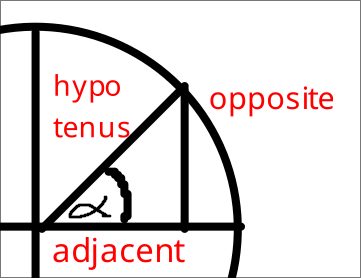
\includegraphics[scale=0.3]{2022-12-29:03:23:18.png}
}[0.25,0.25]

\section{Static}
\subsection{Forces}
\subsubsection{Types}
\vspace{2mm}
\begin{itemize}
\item \textcolor{purple}{movement -> acceleration and braking}
\item \textcolor{purple}{deformation}

\end{itemize}

\subsubsection{Gravity}
\textcolor{purple}{\( |\vec{F_G}| = G * \dfrac{m_1 * m_2}{r^2} \)} | 
G = \(6.67 * 10^{-11}\dfrac{m^3}{kgs^2}\)\vspace{2mm}

\subsubsection{Gravity change}
Difference in some height to surface earth for gravity.\newline
\, \newline
\large \textcolor{purple}{\( \dfrac{F_G}{F_{G0}} = \dfrac{G*\dfrac{m_1 * m_2}{(r_E + h)^2}}{G*\dfrac{m_1 * m_2}{r_E^2}} = \dfrac{\dfrac{G}{(r_E + h)^2}}{\dfrac{G}{r_E^2}}  = \dfrac{r_E^2}{(r_E + h)^2} \)}\newline
\, \newline
\textcolor{orange}{Because the masses appear twice, they can be ignored!}\newline
\, \newline
\normalsize The result is a factor by which the second gravity is lower than the one on earth itself.\newline
Legend: \newline
\begin{itemize}
  \item \(F_G\) = Gravity at new height
  \item \(F_{G0}\) = regular gravity at surface
\item h = height difference
\item \(m_1\) = mass of object 
\item \(m_2\) = mass of earth 
\item G = gravitational constant
\end{itemize} 

\subsubsection{Fall acceleration}
\textcolor{purple}{\(|\vec{F_G}| = m * g\)} | with \(g = 9.81\dfrac{m}{s^2}\)

\subsubsection{Newton}
\textcolor{purple}{\(1N = 1kg * \dfrac{m}{s^2}\)}\vspace{2mm}

\subsection{MassPoint}
\subsubsection{Term Definition} 
A Masspoint is simply a weight without a volume, aka it is the center of mass itself.

\subsubsection{regular friction}
regular friction has 2 formulas. \newline
standing friction = standing coefficient * force of mass \newline
\large \textcolor{red}{\(F_{s} = \gamma_s * F_G\)}\newline 
\normalsize friction = moving coefficient * force of mass \newline 
\large\textcolor{red}{\(F_{m} = \gamma_m * F_G\)} \normalsize\newline
\pic{2022-09-30-11:13:56.png}

\subsubsection{viscose friction}
Viscose friction happens when you do not have a rigid/dry body.\newline
A good example for this are tires. They act as a "lubricant" in proper conditions -> see F1.\newline
In this case the more contact you have to the floor, the less friction you will have.\newline
Interestingly this also means that it is very unlikely that you get stuck in mud/snow with small tires,\newline
but very much likely that you do get stuck with big slick tires -> also see f1 kekw

\subsubsection{Actio \& Reactio}
A force being inflicted upon a body will be met with the same force by said body.\newline
The only difference here is that the body with more mass has more "lag". \newline
In other words, more force is needed to accelerate that body.\newline
This means that the only reason why the earth doesn't follow you when you jump,\newline
is that the earth is by magnitudes heavier than you!\newline
\pic{2022-09-30-11:28:18.png}

\subsubsection{Normal Force}
The normalforce is the experienced counterforce that is applied to an object when being pushed. Eg. the normalforce of an object that is only affected by gravity is just gravity! 

\subsubsection{inclined plane}
\textcolor{orange}{For the inclined plane, we can't directly use gravity as the normalforce, since the incline splits gravity into a relative x and y axis. 
Luckily we can use the \textbf{cos and sin} of the incline angle in order to calculate this!}\newline
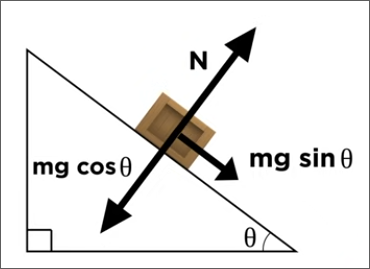
\includegraphics[scale=0.3]{2023_01_03_10_50_26.png}

\subsubsection{rope Force}
\textcolor{purple}{A force that is supported by multiple ropes will split the weight on these ropes.}

\section{torque}
\subsubsection{line of effect}
A vector of a force can be used anywhere on that vector.\newline
This means that the point of effect can be moved infinitely in the vector line.\newline
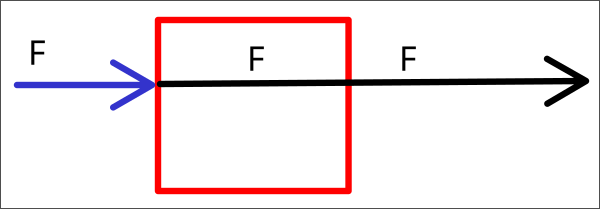
\includegraphics[scale=0.2]{2022-09-30-11:37:46.png}

\subsubsection{lever} 
\minipg{
}{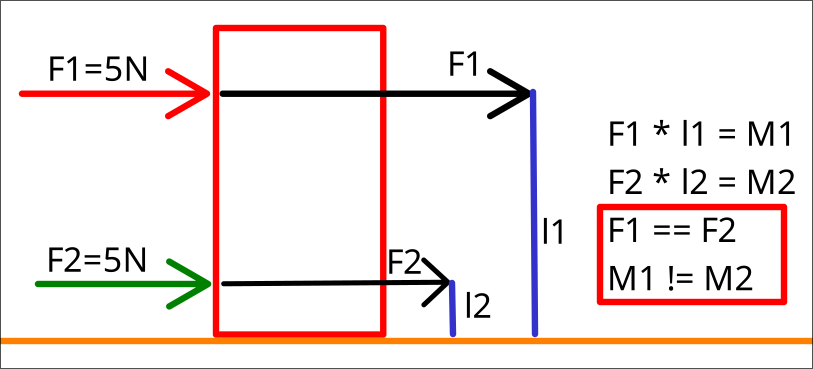
\includegraphics[scale=0.2]{2022-09-30-11:44:32.png}}[0.2,0.2]

\subsubsection{Plank}
\, \newline
\large \textcolor{purple}{\( F_A =\left(\dfrac{l_2}{2}-l_1\right) * F_1 + \left( l_2-l_1-l_3 \right) * F_2\)}\newline
\, \newline
\large \textcolor{purple}{\( F_B = \dfrac{l_2}{2*l_1} * F_1 + \dfrac{l_2 - l_3}{l_1} * F_2 \)}
\, \newline
\normalsize Legend: \newline
\begin{itemize}
\item \(F_1\) = force of plank
\item \(F_2\) = force of object on plank
\item \(l_1\) = length of wall to turning axis point B 
\item \(l_2\) = length of plank
\item \(l_3\) = distance object to plank end 
\end{itemize} 
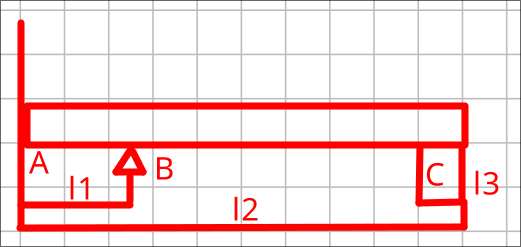
\includegraphics[scale=0.3]{2023_01_03_01_23_30.png}

\subsubsection{Balance}
When keeping an object in balance with torque, keep in mind that you always need the correct angle and attack point!\newline
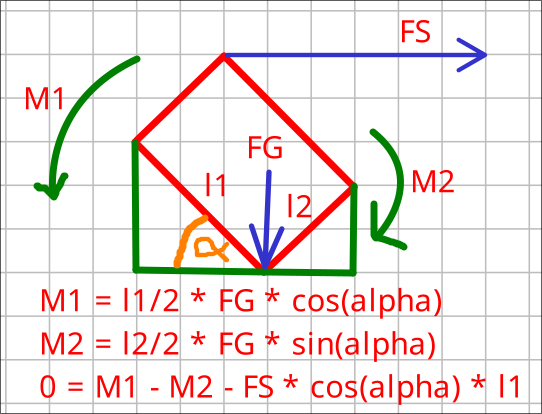
\includegraphics[scale=0.3]{2023_01_03_02_17_17.png}

\subsubsection{Force and Acceleration} 
\textcolor{teal}{A force will always result in an acceleration, this can either be positive or negative(braking).\newline
However remember that an acceleration of 0 does not mean braking, it means constant speed!}

\subsubsection{torque}
\Large \( |\vec{M}| = a * |\vec{F}| \) | Unit: Nm\newline
\, \newline
\textcolor{teal}{ \normalsize \textbf{The value of Torque is always the length * force.}\newline
And it does not matter what constellation of force and length you use\newline
It will always be the same result as when the force increases with a new constellation the length decreases!}\newline
\, \newline
\textbf{Torque in vector format}\newline
It is simply the cross product of 2 vectors!\newline
\pic{2022-10-07-10:47:00.png}\newline
\minipg{
\Large \textcolor{teal}{These 2 can be combined!}\newline
\normalsize \textcolor{teal}{Notice the length and the force F, they have a 90 degree angle as is needed.\newline
\textbf{However the same calculation can be achieved by using the value of the cross product between r and F.\newline
This can be done as long as we have a reference point, here R!.}}\newline
\, \newline}
{\pic{2022-10-07-10:50:19.png}}[0.3,0.2]
\Large if reference point available:\newline \( |\vec{M}| = | \vec{r} \text{x} \vec{F} | = a * | \vec{F} | \ \)

\section{Mass and Equilibrium}

\subsubsection{Center of Mass} 
\minipg{
\textbf{\textcolor{teal}{ The sum of a mass * length -> level over the sum of all masses will result in either the center of mass,\newline
or an axis of it -> x, y, z.}}
}
{
\, \newline
\Large \( x_s = \dfrac{\sum_i x_i * m_i }{\sum_i m_i} \)\newline
\, \newline
\Large \( y_s = \dfrac{\sum_i y_i * m_i }{\sum_i m_i} \)\newline
\, \newline
\Large \( z_s = \dfrac{\sum_i z_i * m_i }{\sum_i m_i} \)\newline}[0.3,0.2]

\subsubsection{Equilibrium}
If you want an equilibrium, then all forces need to combine into 0!\newline
\, \newline
\Large \textcolor{teal}{\( \displaystyle\sum_{n}^{i=1}\vec{F_i} = \vec{0} \) AND \( \displaystyle\sum_{m}^{i=1} \vec{M_i} = \vec{0} \)}\newline
\normalsize 

\subsubsection{Types of Equilibriums}
\begin{itemize}
\item \textcolor{purple}{stable equilibrium}\newline
pushing an item in this state will cause the item to return to the original form.
\item \textcolor{purple}{unstable equilibrium}\newline
Pushing an item in this state will destroy the equilibrium.
\item \textcolor{purple}{indifferent equilibrium}\newline
Pushing an item in this state will create a new equilibrium.

\end{itemize} 

\subsection{Tension, Torsion, Contraction, Compression}
\subsubsection{Pull-Pressure} 
\textcolor{teal}{The pullpressure is the vertical pressure per area.}\newline
\, \newline
\large \( \sigma = \dfrac{F_v}{A} \) | v for vertical\newline
\normalsize 

\subsubsection{Pushpressure} 
\textcolor{teal}{the pushpressure is the parallel pressure per area.}\newline
\, \newline
\large \( \tau = \dfrac{F_p}{A} \) | p for parallel\newline
\normalsize 

\subsubsection{Stretching}
\minipg{
\, \newline
\textcolor{red}{Hook's law}\newline
\textcolor{purple}{This is only applicable if the forces are not too big!}\newline
The stretching is \textbf{similar} to the pullpressure.\newline
This can be visualized via this formula:\newline
\, \newline
\large \( \epsilon = \dfrac{\Delta l}{l} \approx \dfrac{F}{A} = \sigma \) | | | \large \( \epsilon = \dfrac{1}{E} * \sigma \)
\, \newline
\normalsize  Legend:\newline
\begin{itemize}
\item \textcolor{black}{\(\epsilon\) = strain/stretching -> (Dehnung)}
\item \textcolor{black}{E = elastic modulus [\(\dfrac{N}{m^2}\)]}
\item \textcolor{black}{F = Force}
\item \textcolor{black}{\(\sigma\) OR \(\tau\) pressure, see above}
\item l and \(\delta\) l = length and change in length 
\item A = Area/cross-section, \textbf{not} surface area!
\end{itemize}
}{
  Hook's law only applies for forces that are small enough to be withing the proportionality limit, after that the effects are no longer linear!\newline
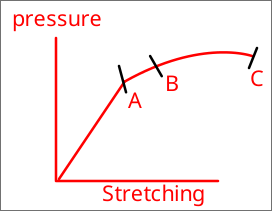
\includegraphics[scale=0.4]{2022-12-29:12:45:07.png}\newline
Point A = Proportionality limit\newline
Point B = Elasticity limit\newline
Point C = Failure Point
}[0.3,0.2]

\subsubsection{Compressability}
\, \newline
\large \( \dfrac{\Delta V}{V} = - \kappa * \Delta p  \)
\, \newline
\, \newline
\large \( \kappa = 0 \text{ or } \text{ -> } \mu = 0.5  \) for a completely rigid body!!
\, \newline
\normalsize Legend:\newline
\begin{itemize}
\item \textcolor{black}{\(\kappa \) = Compressibility Constant}
\item \textcolor{black}{V = Volume}
\item \textcolor{black}{\(\delta V \) = change in Volume}
\item \textcolor{black}{\(\delta p \) = change in Pressure}
\end{itemize} 

\subsubsection{crosscontraction}
\minipg{
\, \newline
\large \( \epsilon_q = \dfrac{\Delta d}{d} \)\newline
\, \newline
\normalsize Legend:\newline
\begin{itemize}
\item \textcolor{black}{d and \(\Delta\)d = diameter and change in diameter}
\item \textcolor{black}{\(\epsilon_d\) = crosscontraction}
\end{itemize} 
}{
This defines that when stretching something like a rod, not only will it grow longer when stretching, it will also be thinner!
}[0.2,0.3]

\subsubsection{crosscontraction as Poisson-Number}
\minipg{
\, \newline
\large \( \epsilon_q = -\mu \epsilon \)\newline
\, \newline
\normalsize Legend: \newline
\begin{itemize}
\item \textcolor{black}{\(\mu\) = Poisson number}
\item \textcolor{black}{\(\epsilon\) = stretching}
\item \textcolor{black}{\(\epsilon_d\) = crosscontraction}
\end{itemize} 
}{
The poisson number \(\mu\) is a unitless property of materials, and usually has a value between 0.15 and 0.5.\newline
It essentially defines how "elastic" a material is.
}[0.18,0.3]

\subsubsection{Torsionmodel}
\minipg{
\, \newline
\large \textcolor{purple}{\( G = \dfrac{E}{2 (1+\mu)} \)}\newline
\, \newline
\normalsize Legend: \newline
\begin{itemize}
\item G = Materialconstant torsion modulo
\item E = elastic modulus
\item \(\mu\) = Poisson Number 
\end{itemize} 
}{
Due to the poisson number being withing 0 to 0.5, the following are the limits for G:\newline
\, \newline
\large \textcolor{purple}{\( \dfrac{E}{3} \le G \le \dfrac{E}{2} \)}\newline
\, \newline
}[0.22,0.25]

\subsubsection{Torsion-Spring}
\, \newline
\large \textcolor{purple}{\( \phi = \dfrac{M}{c} = \dfrac{M * 2l}{\pi * G * r^4} = \dfrac{M * 2l}{\pi * \dfrac{E}{2 (1 + \mu)} * r^4} = \dfrac{M * 4l * (1 + \mu)}{\pi * E * r^4}\)}\newline
\, \newline
\normalsize 
\minipg{
Legend: \newline
\begin{itemize}
\item M = torque
\item c = ??
\item \(\phi\) = turning angle 
\item l = length
\end{itemize} 
}{
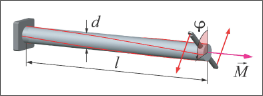
\includegraphics[scale=0.4]{2022-12-29:01:16:07.png}
}[0.25,0.25]\newline
for a completely rigid body: \(\mu = 0.5\) | \(G = \dfrac{E}{3}\) | \(E = \infty\)\newline
something over infinity will be 0 when considering the limit

\subsubsection{Screw-Spring}
\, \newline
\large \textcolor{purple}{\( \Delta l = \dfrac{F}{c} = \dfrac{F * 4nR^3}{G * r^4} = \dfrac{F * 8nR^3 (1 + \mu)}{E * r^4}\)}\newline
\, \newline
\normalsize 
\minipg{
Legend: \newline
\begin{itemize}
\item F = force
\item c = ??
\item l = length
\item n = amount of coils
\item R = radius of coil
\end{itemize} 
}{
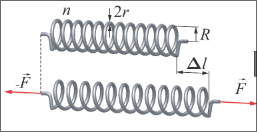
\includegraphics[scale=0.4]{2022-12-29:01:30:58.png}
}[0.25,0.25]\newline
for a completely rigid body: \(\mu = 0.5\) | \(G = \dfrac{E}{3}\) | \(E = \infty\)\newline
something over infinity will be 0 when considering the limit

\subsubsection{Plankdeformation}
\minipg{
\, \newline
\large \textcolor{purple}{\( z = \dfrac{4 * l^3}{E * b * h^3} \)}\newline
\, \newline
\normalsize Legend: \newline
\begin{itemize}
\item z = change in height
\item b = ??
\item h = height 
\item E = elastic modulo
\end{itemize} 
}{
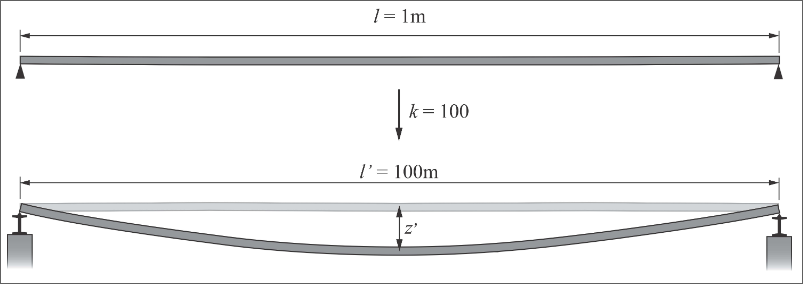
\includegraphics[scale=0.2]{2022-12-29:01:32:42.png}\newline
This picture simply states that we can scale this from 1m to 100m
}[0.20,0.25]\newline
\(z = \frac{5\cdot 7800\,\mathrm{kg}/\mathrm{m}^3\cdot 9.81\,\mathrm{m}/\mathrm{s}^2\cdot 1\,\mathrm{m}^4}{32\cdot 2\cdot 10^{11}\,\mathrm{N}/\mathrm{m}^2 \cdot \left(0.01\,\mathrm{m}\right)^2} \approx 5.98\cdot10^{-4}\,\mathrm{m} = 0.598\,\mathrm{mm}\quad\)\newline
100m -> 5.98m | only the \((1m)^4\) changes to \((100m)^4\)


\section{kinematic}
\subsection{Median acceleration}
\textcolor{orange}{The median acceleration is the end velocity - the start velocity over the end time - the start time:}\newline
\, \newline
\large \( \overset{\_}{a} = \dfrac{v_2 - v_1}{t_2 - t_1} = \dfrac{v(t_2) - v(t_1)}{t_2 - t_1} \) \newline
\normalsize 

\subsubsection{Current Acceleration}
\textcolor{orange}{The current acceleration is the limit of the current velocity - the velocity of current time - delta time over delta time. \newline
Or easier, the derivation of current velocity:}\newline
\, \newline
\large \( a(t) = \underset{\Delta t -> 0}{\lim} \dfrac{v(t) - v(t - \Delta t)}{\Delta t} = \dfrac{d}{dx}v(t)\) \newline
\normalsize

\subsubsection{Derivatives}
\, \newline
\large \(\dfrac{d}{dt}a(t) = v(t) = \int{s(t)} \)\newline
\, \newline
\large \(\dfrac{d}{dt}v(t) = s(t)\)\newline
\, \newline
\normalsize \textcolor{orange}{Also note that when you integrate, you get a constant c -> hence the following:}\newline
\, \newline
\large \( v(t) = \int{a(t) dt} = \int{0 dt} = c \text{ --> if a(t) == 0}\) \newline
\, \newline
\normalsize \textcolor{red}{This is why the acceleration on earth -> gravity is constant!! HOLY FUCK}

\subsubsection{Derivative of a Vector}
\textcolor{orange}{The derivative of a vector is the derivative of each component, meaning the following:}\newline
\large \(\dfrac{d}{dx} \vec{r}(t) = (\dfrac{d}{dx} x(t), \dfrac{d}{dx} y(t), \dfrac{d}{dx} z(t) ) \)\newline
\, \newline \normalsize

\subsubsection{Current Velocity with Vectors}
\textcolor{orange}{This specifies the current velocity of a vector:}\newline
\, \newline
\large \( \vec{v}(t) = \underset{\Delta t -> 0}{\lim} \dfrac{\Delta \vec{r}}{\Delta t} = \dfrac{d}{dx} \vec{r} = \overset{.}{\vec{r}} \) \newline 
\, \newline \normalsize

\subsubsection{Equal accellerated translation}
\, \newline
\large \textcolor{purple}{\( a(t) = a_0 \) OR \(a = \dfrac{\Delta v}{\Delta t} [\dfrac{m}{s^2}]\) }\newline
\, \newline
\large \textcolor{purple}{\( v(t) = \int{a_0 dt} = a_0 * t + c_1 \) OR \(v(t) = v_0 + a * t\)}\newline
\, \newline
\large \textcolor{purple}{\( x(t) = \int{\int{ a_0 dt }} = \int{a_0 * t + c_1 dt} = \dfrac{1}{2}* a_0 * t^2 + c_1 * t + c_2\)}\newline
\, \newline
\large \textcolor{purple}{\( x(t) = v_0 * t + \dfrac{a * t^2}{2} \)}\newline
\, \newline
\normalsize 

\subsubsection{Equally de-accelerated Translation}
\, \newline
\large \textcolor{purple}{\( a = \dfrac{v^2}{2s} \)}\newline
\, \newline
\large \textcolor{purple}{\( s = \dfrac{v^2}{2 * \mu * G} \)}
\, \newline
\normalsize Legend: \newline
\begin{itemize}
\item s = distance to v == 0 (braking)
\item a = deacceleration\newline
\textcolor{red}{Keep in mind this needs to be negative compared to the velocity!}
\item \(\mu\) = friction coefficient
\item G = gravitational constant
\item v = velocity
\end{itemize} 

\subsubsection{extreme values}
In order to get the maximum of a parabel, you have 2 possibilities, either set the acceleration to 0 which can be calculated by getting the initial acceleration and then reducing it with gravity until you find the proper time:\newline
\, \newline
\Large \textcolor{purple}{\(t_{\text{max}} = \dfrac{\dfrac{sin(\alpha) F}{m} - g}{g}\) | \(a_{\text{vertical}} = \dfrac{sin(\alpha) * F}{m}\)}
\, \newline
\textcolor{purple}{\( v_0 = a_{\text{vertical}} - g \) | \( 0 = v_0 - t_{max} * g \)} 
\newline
Or you can set the slop of x to 0 with derivations:\newline
\, \newline
\large \textcolor{purple}{\( x(tmax) = -\dfrac{1}{2}g * t^2_{max} + v_0 * t_{max} + h_0\)}\newline
\, \newline

\subsubsection{osculating circle (Schmieg)}
This is a circle that in respect to 3 points will go through all of them in the trajectory of an object.\newline
It is used to get a radius that is needed in order to calculate the speed, acceleration etc.\newline
\minipg{
\, \newline
\large \textcolor{purple}{\(  
			\vec{a} = \frac{\mathrm{d}}{\mathrm{d}t}\vec{v} = \lim\limits_{\Delta t \rightarrow 0}\frac{\vec{v}\left(t+\Delta t\right)-\vec{v}\left(t-\Delta t\right)}{\Delta t} \quad\) \newline
		where \(t_1 = t-\Delta t\) und \(t_2 = t+\Delta t\)}\newline
\, \newline
\normalsize 
}{
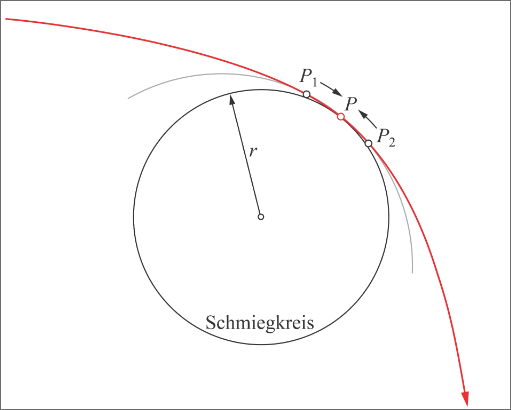
\includegraphics[scale=0.2]{2022-12-29:04:06:04.png}
}[0.3,0.25]

\subsubsection{Radial and Tangential Acceleration}
\textcolor{red}{Tangential Acceleration is the speed of the object -> \(|\vec{v}|\)}\newline
\textcolor{red}{Radial Acceleration is the direction of the object -> \(\vec{v}\)}\newline
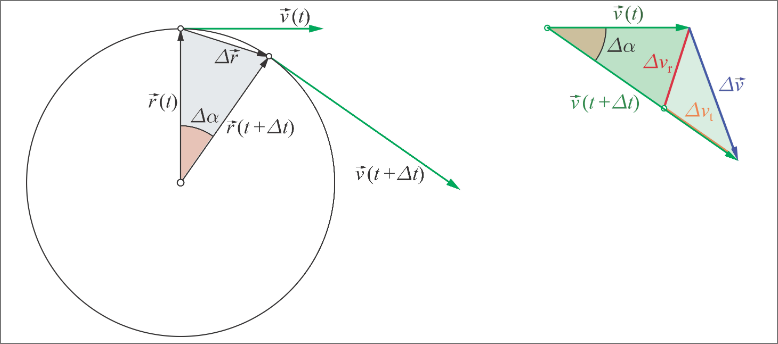
\includegraphics[scale=0.2]{2022-12-29:04:15:14.png}\newline
\, \newline
\large \( a_{tan} = \underset{\Delta t -> 0}{lim} \dfrac{\Delta v_{tan}}{\Delta t} = \dfrac{dv}{dt} = \overset{.}{v} \) \newline
\, \newline
\large \( \dfrac{\Delta v_{rad}}{v} = \dfrac{\Delta r}{r}\) ==> \( a_{rad} = \underset{\Delta t -> 0}{\lim} \dfrac{\Delta v_{rad}}{\Delta t} = \dfrac{v}{r}\underset{\Delta t -> 0}{\lim} \dfrac{\Delta v}{\Delta t} = \textcolor{red}{\dfrac{v^2}{r}} \) \newline
\, \newline \normalsize

\subsubsection{Equally accelerated tangential translation}
\, \newline
\large \textcolor{purple}{\( v(t) = a_{tan} * t + v_0 \)}\newline
\large \textcolor{purple}{\( s(t) = \dfrac{a_{tan} * t^2}{2} + v_0 * t + s_0\)} \newline
\, \newline \normalsize \
\textcolor{orange}{In case that \(a_{tan}\) is 0, you obviously only evaluate \(v_0 * t + s_0\) , this is because the first part would evaluate to 0.}

\subsubsection{Coordinates}
\(\text{Kartesian Coordinates:} \quad\vec{P}= \begin{pmatrix}x\\y \end{pmatrix} = \begin{pmatrix}r\cdot \cos\phi\\ r\cdot \sin\phi\end{pmatrix}\quad \newline
\text{Polar Coordinates:} \quad\vec{P}= \begin{pmatrix}r\\ \phi \end{pmatrix} = \begin{pmatrix}\left|\sqrt{x^2+y^2}\right|\\ \tan\frac{y}{x}\end{pmatrix}\quad\)

\subsubsection{Angle Velocity}
\, \newline
\large \textcolor{purple}{\( \omega = \underset{\Delta t -> 0}{\lim} \dfrac{\phi(t + \Delta t) - \phi(t)}{\Delta t} = \dfrac{d\phi}{dt} = \overset{.}{\phi} \)} | 
\large \textcolor{purple}{\( \phi = \dfrac{s}{r} \)}\newline
\large \textcolor{purple}{\( v = \frac{\mathrm{d}s}{\mathrm{d}t} = \frac{\mathrm{d}s}{\mathrm{d}t} = \underbrace{\frac{\mathrm{d}r}{\mathrm{d}t}}_{=0} \phi + r\frac{\mathrm{d}\phi}{\mathrm{d}t} = r\omega\quad\)}
\, \newline \normalsize
\begin{itemize}
\item \textcolor{orange}{\(\phi\) == angle}
\item \textcolor{orange}{\(\omega\) == angle acceleration}
\item \textcolor{orange}{ t == time}
\item \textcolor{orange}{s == distance}

\end{itemize}

\subsubsection{Frequency and Circulation}
\minipg{
\, \newline
\large \textcolor{purple}{\( f = \dfrac{1}{T} <=> T = \dfrac{1}{f} \)}\newline
\, \newline
\large \textcolor{purple}{\( \omega = \dfrac{2\pi}{T} <=> T = \dfrac{2\pi}{\omega} \)}\newline
\, \newline \normalsize
}{
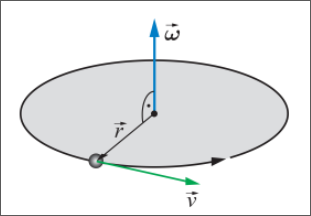
\includegraphics[scale=0.3]{2022-12-29:04:36:50.png}
}[0.25,0.25]
\, \newline
\large \textcolor{purple}{\( \omega = 2\pi f <=> f = \dfrac{\omega}{2\pi} \)}\newline
\, \newline
\large \textcolor{orange}{\( r \omega = \dfrac{2\pi r}{T} = v \)}\newline
\, \newline
\large \textcolor{orange}{\( \alpha = \underset{\Delta t -> 0}{\lim} \dfrac{\omega (t + \Delta t) - \omega (t)}{\Delta t} = \dfrac{d\omega}{dt} \)}\newline 
\, \newline
\large \textcolor{orange}{\( \alpha_{tan} = \dfrac{dv}{dt} = \dfrac{d}{dt}r * \omega = r * \alpha \)}\newline 
\, \newline
\textcolor{purple}{constant angle-motion (no acceleration)}\newline
\large \textcolor{orange}{\( \Phi(t) = \omega_0 * t + \Phi_0 \)  | given \(\alpha == 0 \) and \( \omega = \omega_0 == \text{ constant} \)}\newline
\, \newline
\textcolor{purple}{constant accelerated angle-motion}\newline
\large \textcolor{orange}{\( \Phi(t) = \dfrac{\alpha_0 t^2}{2} + \omega_0 * t + \Phi_0 \) \newline given \( \alpha == \alpha_0 == \text{ constant} \) and \(\omega == \alpha_0 * t + \omega_0 \) }\newline
\, \newline \normalsize
\begin{itemize}
\item \textcolor{orange}{T = Time per Circulation}
\item \textcolor{orange}{\(f\) == frequency}
\item \textcolor{orange}{r == radius}
\item \textcolor{orange}{v == velocity}
\item \textcolor{orange}{\(\Phi\) == angle}
\item \textcolor{orange}{\(2\pi\) == 1 Circulation}
\end{itemize}

\subsection{Free Fall and Parables}
\subsubsection{Vertical Throw}
\, \newline
\large \textcolor{orange}{\( \alpha = -g == \text{ constant}  \)}\newline
\, \newline
\large \textcolor{orange}{\( v(t) = -g * t + v_0 \)}\newline
\, \newline
\large \textcolor{orange}{\( h(t) = \dfrac{-g * t^2}{2} + v_o * t + h_0  \)}\newline
\, \newline
\large \textcolor{purple}{\( t_{max} = \dfrac{v_0}{g} \)}\newline
\, \newline
\large \textcolor{purple}{\( h_{max} = h(t_{max}) = \dfrac{-g * v^{2}_{0}}{2 g^2 } + \dfrac{v_{0}^{2}}{g} + h_0 = \dfrac{v_{0}^{2}}{2g} + h_0 \)}\newline
\, \newline \normalsize
\begin{itemize}
\item \textcolor{orange}{a == acceleration}
\item \textcolor{orange}{v = velocity}
\item \textcolor{orange}{h = height}
\item \textcolor{orange}{t = time}
\item \textcolor{orange}{g = gravity -> 9.81}
\end{itemize} 

\subsubsection{Free Fall}
\, \newline
\large \textcolor{orange}{\( a = -g == \text{ constant} \)}\newline
\, \newline
\large \textcolor{orange}{\(v(t) = -g * t\)}\newline
\, \newline
\large \textcolor{orange}{\(h(t) = \dfrac{-g * t^2}{2} + h_0\)}\newline
\, \newline \normalsize
\begin{itemize}
\item \textcolor{orange}{a == acceleration}
\item \textcolor{orange}{v = velocity}
\item \textcolor{orange}{h = height}
\item \textcolor{orange}{t = time}
\item \textcolor{orange}{g = gravity -> 9.81}
\end{itemize} 

\subsubsection{Diagonal Throw}
Remember that the y-axis is sine * angle, and the x-axis is cos * angle\newline
\minipg{
\large \textcolor{purple}{\( v_x = v_0 * cos(\alpha) \)}\newline
\large \textcolor{purple}{\( v_y = v_0 * sin(\alpha) \)}\newline
\large \textcolor{purple}{\( v_0 = a_0 - g \)}\newline
\large \textcolor{purple}{\( a_0 = \dfrac{F}{m}\)}\newline
\, \newline
\normalsize Legend: \newline
\begin{itemize}
\item \(v_x\) = \(v_0\) in x direction
\item \(v_y\) = \(v_0\) in y direction
\item \(a_0\) =  initial acceleration of throw
\item \(\alpha\) = angle of throw
\end{itemize} 
}{
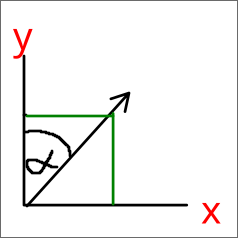
\includegraphics[scale=0.4]{2022-12-29:04:46:12.png}
}[0.25,0.25]
\, \newline

\subsubsection{Maximal Throw Gravity at new heightdistance}
We evaluate the angle via settings the slope of the derivative to 0. :)\newline
\minipg{
\, \newline
\large \textcolor{purple}{\( 0\overset{!}{=}\frac{\mathrm{d}x_\text{max}}{\mathrm{d}\alpha} = \frac{v_0^2}{g}\cos\left(2\alpha\right)\cdot 2 \) \newline \(\alpha \in\{45^\circ,135^\circ\}\quad \)}\newline
\, \newline
\normalsize 
}{
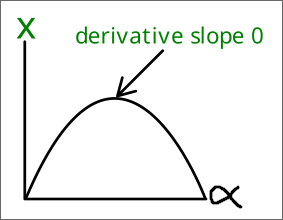
\includegraphics[scale=0.4]{2022-12-29:04:55:07.png}
}[0.25,0.25]

\subsubsection{Angle given explicit Throwdistance}
\, \newline
\large \textcolor{purple}{\(
\alpha = \frac{1}{2}\arcsin\frac{g\cdot d}{v_0^2}
  \)}\newline
\, \newline

\section{Dynamic}

\subsection{Newtons Laws}
\begin{enumerate}
\item \textcolor{purple}{Law of Inertia}\newline 
All mass is inert, meaning that it will keep the same velocity unless a force is acted upon it
\item \textcolor{purple}{Law of Action}\newline
  \(\vec{F} = m * \vec{a}\)
\item \textcolor{purple}{ExchangeForce}\newline
  If two bodies exert forces on each other, these forces have the same magnitutde but opposite directions
\end{enumerate} 

\subsection{Friction Forces}
\subsubsection{Gliding Friction}
\textcolor{red}{This Force is opposite to the propelling force!}\newline
\, \newline
\large \textcolor{purple}{\( F_R = \mu_G * F_N \)}\newline
\, \newline
\normalsize Legend: \newline
\begin{itemize}
\item \(F_R\) = Force to exceed with Gliding
\item \(F_N\) = Normal Force -> 90 degree to surface -> not always equal to gravity
\item \(\mu_G\) = Gliding friction coefficient
\end{itemize} 

\subsubsection{RollFriction}
\textcolor{red}{This Force is opposite to the propelling force!}\newline
\minipg{
\, \newline
\large \textcolor{purple}{\( F_R = \mu_R * F_N \)}\newline
\, \newline
\normalsize Legend: \newline
\begin{itemize}
\item \(F_R\) = Force to exceed with Gliding
\item \(F_N\) = Normal Force -> 90 degree to surface -> not always equal to gravity
\item \(\mu_R\) = Rolling friction coefficient
\end{itemize} 
}{
  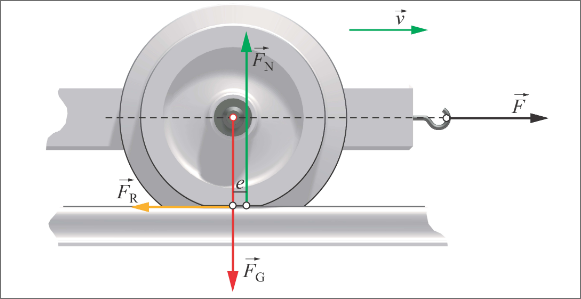
\includegraphics[scale=0.2]{2022-12-29:05:25:34.png}
}[0.25,0.25]

\subsubsection{RollFriction Length}
Due to the deformation of a wheel, there is a small length of the wheel that touches the ground. \newline
In other words more than 0mm :) \newline
Hence the normalforce \(F_N\) will be slightly offset.\newline
In order for the wheel to still have a balance, the following must be given:\newline
\, \newline
\large \textcolor{purple}{\( e * F_N - r * F \overset{!}{=} 0 \)}\newline
\, \newline \normalsize
0 would indicate no movement.\newline
\, \newline
\large \textcolor{purple}{\( e = \dfrac{r * F}{F_N} = \dfrac{r * F_R}{F_N} = \dfrac{r * \mu_R * F_N}{F_N} = \mu_R * r \)}
\, \newline \normalsize

\subsection{Work, potential and kinetic Energy}

\subsubsection{Unit of Work}
The unit of work is \(Nm\), but because of the potential confusion, we use the unit \(J\) for \textbf{Joule} instead!

\subsubsection{Work with constant Force}
\minipg{
\, \newline
\large \textcolor{purple}{\( W = F_s * s_{AB} \)}\newline
\, \newline
\normalsize
}{
Legend: \newline
\begin{itemize}
\item W = Work
\item \(F_s\) = Force for this specific length
\item \(s_AB\) = part of the whole distance
\end{itemize} 
}[0.25,0.25]

\subsubsection{Work with non constant Force}
\minipg{
\, \newline
\large \textcolor{purple}{\( W = \int^B_A{dW} = \int^B_A{\vec{F} * d\vec{s}} \)}\newline
\, \newline
\normalsize Legend: \newline
\begin{itemize}
\item W = Work 
\item F = Force
\item s = distance
\end{itemize} 
}{
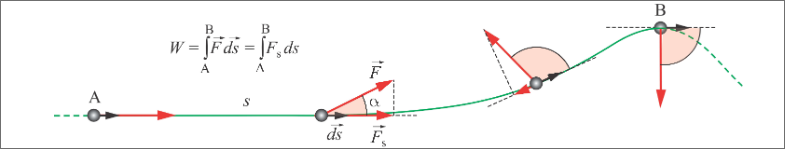
\includegraphics[scale=0.2]{2022-12-29:05:45:58.png}
}[0.20,0.25]\newline
\textcolor{purple}{The problem here is that we have different forces depending on where on s we are located}

\subsubsection{Potential Energy}
\textcolor{purple}{These are energies that are essentially "stored", ex. a book that I hold can fall down, which is "work".\newline
Or a spring that I compressed has the potential to jump into it's original shape -> which is "work"}\newline
\, \newline
\large \textcolor{purple}{\( W = m * g * h \)}\newline
\, \newline
\normalsize Legend: \newline
\begin{itemize}
\item W = Work (here potential Work)
\item m = mass
\item g = gravity 
\item h = height
\end{itemize}

\subsubsection{Potential Energy with Springs}
\minipg{
\, \newline
\large \textcolor{purple}{\( F = -k * x \)}\newline
\large \textcolor{purple}{\( W = \int^{x_0}_0{-F * dx} = \int^{x_0}_0{k * x * dx} = \dfrac{k * x^2_0}{2}\)}\newline
\, \newline
\normalsize Legend: \newline
\begin{itemize}
\item F = Force used to prepare spring
\item k = Springconstant
\item x = length that was stretched or compressed 
\item W = potential Energy
\end{itemize} 
}{
  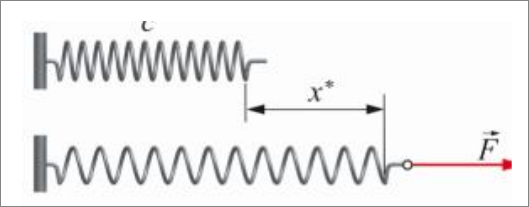
\includegraphics[scale=0.25]{2022-12-29:06:12:50.png}
}[0.25,0.25]

\subsubsection{Conservation Law}
\textcolor{purple}{When working within a closed system, ALL energy is preserved, it is simply transformed.\newline
For example when picking up a stone and then letting it fall, the entire energy is the same, aka E total is always the sum of E potential and E kinetic!}\newline
\, \newline
\large \textcolor{purple}{\( E_{\text{pot}} + E_{\text{kin}} = E_{\text{tot}} = \text{constant}\)}\newline
\, \newline
\normalsize 

\subsection{Power and Power coefficient}
\minipg{
\, \newline
\large \textcolor{purple}{\( P = \dfrac{\Delta W}{\Delta t} = \dfrac{\vec{F}*\Delta\vec{s}}{\Delta t}  = \vec{F}*\vec{v} \)}\newline
\, \newline
\large \textcolor{purple}{\( \eta = \dfrac{P_{\text{in}}}{P_{\text{out}}} \)}
\, \newline
\normalsize 
}{
Legend: \newline
\begin{itemize}
\item W = Work
\item P = Power
\item s = distance 
\item v = velocity
\item \(\eta\) = power coefficient 
\end{itemize} 
}[0.25,0.25]

\subsection{Impulses and Impulsretention}
\subsubsection{Impulse}
\, \newline
\large \textcolor{purple}{\( \vec{p} = m * \vec{v} \)}\newline
\, \newline
\textcolor{purple}{\( \vec{F} = m\vec{d} = m * \dfrac{d\vec{v}}{dt} = \dfrac{d}{dt} * (m\vec{v}) = \dfrac{d\vec{p}}{dt} \)}\newline
\normalsize \, \newline

\subsubsection{Force Push (kekw-wars)}
\minipg{
\, \newline
\large \textcolor{purple}{ \(\int^{t+\delta t}_{t} F(t) dt = \vec{F}* \delta t = \delta p\)}\newline
\normalsize \, \newline
}{
  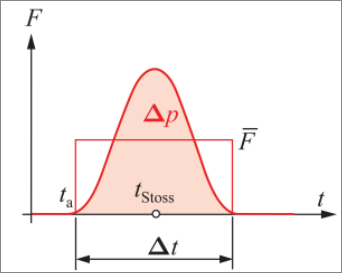
\includegraphics[scale=0.3]{2022_12_31_03_16_05.png}
}[0.25,0.25]

\subsubsection{Impulsretention}
\, \newline
\large \textcolor{purple}{ \( \vec{p} = \int \dfrac{dp}{dt} dt = c \text{ => constant}\)}\newline
\Large \, \newline
Note, \(\dfrac{dp}{dt}\) is 0, therefore in a completely isolated system, the impulse retention is always \textbf{constant!} \normalsize \newline


\subsection{Center of Mass and Impulses} 
\subsubsection{Center of Mass in a collision}
\vspace{2mm}
\large \textcolor{purple}{\( m_1 * \vec{r_1} + m_2 * \vec{r_2} = \vec{0} \text{ <=> } m_1*\vec{v_1} + m_2 * \vec{v_2} = \vec{0} \)}\newline
\normalsize \, \newline
Types of collisions:\newline
\begin{itemize}
\item \textcolor{orange}{straight: the vectors of the center of mass are on one straight line}
\item \textcolor{orange}{tilted: The vectos of the center of mass complete an angle}
\item \textcolor{orange}{central: The center of mass of each collision entity is on the collision normal}
\item \textcolor{orange}{excentric: The center of mass of each collision entity is NOT on the collision normal }
\item \textcolor{orange}{elastic: The total kinetic energy before and ater the collision are the same}
\item \textcolor{orange}{inelastic: The total kinetic energy before and after the collision are different}
\item \textcolor{orange}{completely inelastic: The collision entities move at the same speed after the collision}
\end{itemize} 

\subsubsection{Deformation"Work"}
\vspace{2mm}
\large \textcolor{purple}{\( Q = (E_1 + E_2) - (E_1' + E_2') \geq 0 \)}\newline
\normalsize \, \newline
Legend:\newline
\begin{itemize}
\item \textcolor{orange}{\( E_1 + E_2 =\) Energy before collision}
\item \textcolor{orange}{\( E_1' + E_2' =\) Energy after collision}
\item \textcolor{orange}{Q = DeformationWork}
\end{itemize} 

\subsubsection{Elasticity Count}
\vspace{2mm}
\large \textcolor{purple}{\( k = \dfrac{v_2' - v_1'}{v_1 - v_2} \)}\newline
\normalsize \, \newline
Legend:\newline
\begin{itemize}
\item \textcolor{orange}{\(v_1\) = velocity of entity 1}
\item \textcolor{orange}{\(v_2\) = velocity of entity 2}
\item \textcolor{orange}{k = elasticity count}
\end{itemize} 


\subsection{straight, central, completely elastic collision}

\subsubsection{Impulse Law}
\vspace{2mm}
\large \textcolor{purple}{\( p \overset{!}{=} p' \text{ <=> } m_1v_1 + m_2v_2 \overset{!}{=} m_1v_1' + m_2v_2' \)}\newline
\normalsize \, \newline
Legend:\newline
...

\subsubsection{Energy Law}
\vspace{2mm}
\large \textcolor{purple}{\( E_{\text{kin}} \overset{!}{=} E_{\text{kin}}' \text{ <=> } \dfrac{m_1v_1^2}{2} + \dfrac{m_2v_2^2}{2} \overset{1}{=} \dfrac{m_1v_1'^2}{2} + \dfrac{m_2v_2'^2}{2} \)}\newline
\normalsize \, \newline
\minipg{
Legend:\newline
...
}{
  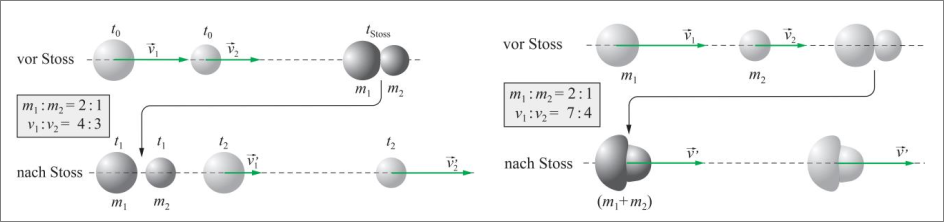
\includegraphics[scale=0.265]{2022_12_31_03_28_29.png}
}[0.05,0.25]

\subsubsection{Special case with \(m_1 = m_2\)}
\vspace{2mm}
\large \textcolor{purple}{\( v_1' = 0 + 1 * 0 = 0 \)}\newline
\textcolor{purple}{\( v_2' = v_1 + 0 = v_1\)}\newline
\normalsize \, \newline
Legend: \newline
...


\subsection{Straight, central, completely inelastic collision}

\subsubsection{Impulse Law}
\vspace{2mm}
\large \textcolor{purple}{\( m_1v_1 = m_2v_2 = (m_1 + m_2 )v' \text{ => } v' = \dfrac{m_1v_1 + m_2v_2}{m_1 + m_2}\)}\newline
\textcolor{red}{\( p = p' \)!!}\newline
\normalsize \, \newline
Legend:\newline
...

\subsubsection{Energy Law and Deformation-Work}
\vspace{2mm}
\large \textcolor{purple}{\( \dfrac{m_1v_1^2}{2} + \dfrac{m_2v_2^2}{2} = \dfrac{(m_1 + m_2)v'^2}{2} + Q \)}\newline
\, \newline
\textcolor{purple}{\(Q = \dfrac{m_1m_2}{2(m_1+m_2)}*(v_1 -v_2)^2\)}\newline
\normalsize \, \newline
Legend:\newline
\begin{itemize}
\item \textcolor{orange}{\(m_1\) = Center of mass entity 1}
\item \textcolor{orange}{\(m_2\) = Center of mass entity 2}
\item \textcolor{orange}{\(v_1\) = velocity entity 1}
\item \textcolor{orange}{\(v_2\) = velocity entity 2}
\item \textcolor{orange}{Q = Deformation-Work}
\end{itemize}


\subsubsection{Reduced Mass, Relative Velocity}
\minipg{
\, \newline
\large \textcolor{purple}{\(v_{\text{rel}} = | v_1 - v_2|\)}\newline
\, \newline
\textcolor{purple}{\(\mu = \dfrac{m_1m_2}{m_1 + m_2}\)}\newline
\, \newline
\textcolor{purple}{\( Q = \dfrac{\mu v_{\text{rel}^2}}{2}\)}\newline
\, \newline
\normalsize 
}{
Legend:\newline
\begin{itemize}
\item \textcolor{orange}{\(v_1\) = velocity entity 1}
\item \textcolor{orange}{\(v_2\) = velocity entity 2}
\item \textcolor{orange}{\(\mu\) = reduced mass}
\item \textcolor{orange}{Q = DeformationWork}
\item \textcolor{orange}{\(v_{\text{rel}}\) = relative velocity}
\end{itemize}
}[0.25,0.25]

\subsubsection{Trace Speed}
\, \newline
\large \textcolor{purple}{\( mv = mv + dm * v + m * dv + dm * dv + dm * u - dm * v \)}\newline
\, \newline
\large \textcolor{purple}{\( 0 = m * dv + dm * u =+ dm * dv \)}\newline
\, \newline
\large \textcolor{purple}{\(	\mathrm{d}v = -u \frac{1}{m}\mathrm{d}m \quad\Rightarrow\quad v = \int\mathrm{d}v = -u\int\frac{1}{m}\mathrm{d}m = -u\ln\left(m\right)+c\)}\newline
\, \newline
\(	t=0\): \(v=v_0\), \(m=m_0\) ==> \(  	c = v_0+u\ln\left(m_0\right) \)\newline
\minipg{
\, \newline
\large \textcolor{purple}{\( 0 \approx dm * dv \)}\newline
\, \newline
\large \textcolor{purple}{\( m * dv = -u * dm \)}\newline
\, \newline
\large \textcolor{purple}{\( \dfrac{dv}{dm} = - \dfrac{u}{m} \)}\newline
\, \newline
}{
\normalsize Legend: \newline
\begin{itemize}
\item u = Trace speed
\item dt = Time interval
\item dm = mass of fuel
\item dv = velocity at interval -> v(dt)
\item m = rest of mass
\end{itemize} 
}[0.25,0.25]
\, \newline
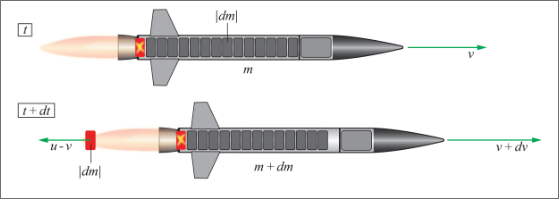
\includegraphics[scale=0.3]{2022_12_31_04_23_57.png}

\subsubsection{Rocket Equation}
\, \newline
\large \textcolor{purple}{\( v(t) = -u * ln(m) + v_0 + u * ln(m_0) = v_0 + u * ln\left(\dfrac{m_0}{m}\right) \)}\newline
\, \newline
\normalsize Legend: \newline
\begin{itemize}
\item \(m_0\) = mass at start
\end{itemize} 

\subsection{Gravity}
\subsubsection{Keplers Laws}
\begin{enumerate}
\item \textcolor{purple}{Planets move on ellipses which surround the sun}\newline
  an ellipses has two \textbf{foci} which are the 2 centers of the ellipses, the sun will be situated in one of these foci!
\item \textcolor{purple}{Each area that the view from the sun to the planet that moves creates, is the same on each point on the orbit}\newline
  \minipg{
  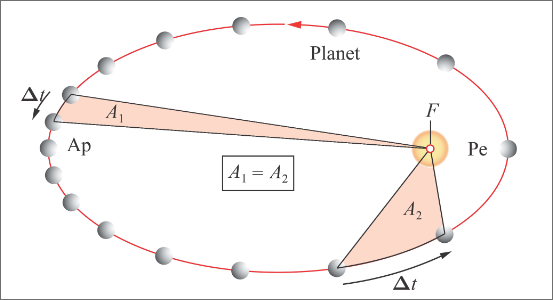
\includegraphics[scale=0.2]{2022_12_31_04_35_35.png}\newline
  }{
  \textcolor{red}{This means that when on the point that is further away from the sun, the planet \textbf{travels slower} than when on the side that is closer!}
  }[0.20,0.25]
\item \textcolor{purple}{the cube of the \textbf{semi-major axis a} is proportional to the square of the \textbf{orbital period} P}\newline
  \minipg{
  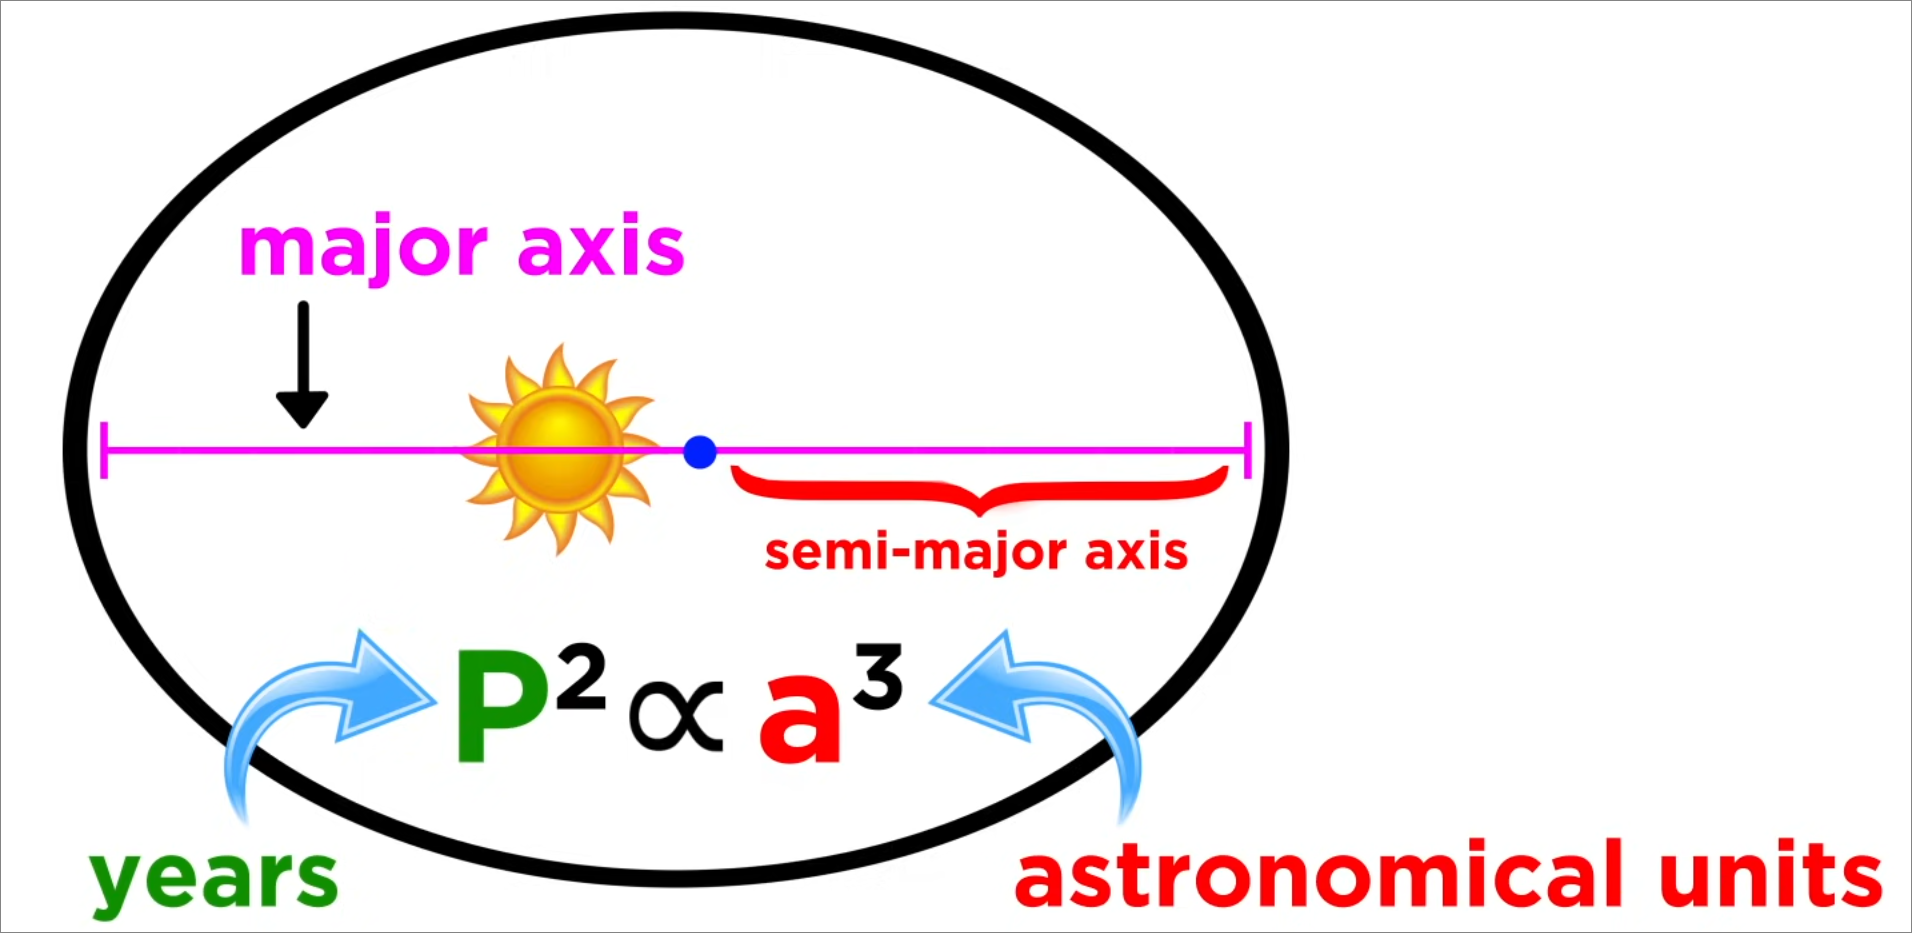
\includegraphics[scale=0.08]{2022_12_31_04_42_59.png}
  }{
  the smaller side of the major axis is the semi-major axis\newline
  Distance measured in AE Astronimical Unit \newline
  \textcolor{purple}{\(1AE == 149.6 * 10^6 \)km}
  \textcolor{purple}{\(a_1 = \left(\dfrac{P_1}{P_2}\right)^\frac{2}{3} * a_2\)}\newline
  \(a_1\) = semi-major axis planet 1\newline
  \(a_2\) = semi-major axis planet 2\newline
  \(P_1\) = Orbit-interval planet 1\newline
  \(P_2\) = Orbit-interval planet 2\newline
  }[0.28,0.20]
\end{enumerate} 

\subsubsection{Gravitational Constant}
\, \newline
\large \textcolor{purple}{\( G = 6.67 * 10^{-11}*\dfrac{m^3}{kg * s^2} \)}\newline
\, \newline
\normalsize 


\subsubsection{Newtons Law of Gravity}
\, \newline
\large \textcolor{purple}{\( F_G = G * \dfrac{m_1m_2}{r^2} \)}\newline
\, \newline
\normalsize Legend: \newline
\begin{itemize}
\item G = Gravitational Constant
\item \(m_1\) = first mass
\item \(m_2\) = second mass
\item r = radius of second object 
\end{itemize} 


\subsubsection{Gravitational Pull -> a ball}
\, \newline
\textcolor{orange}{Within a ball}\newline
\, \newline
\large \textcolor{purple}{\( F_G = G * \dfrac{4 \pi * r^3 * \rho * m}{3r^2} = \dfrac{4 \pi}{3}G \rho m r \)}\newline
\, \newline
\textcolor{orange}{Outside a ball}\newline
\, \newline
\large \textcolor{purple}{\( F_G = G \dfrac{M * m}{r^2} \)}\newline
\, \newline
\normalsize 
\minipg{
Legend: \newline
\begin{itemize}
\item G = gravitational constant
\item r = radius
\item \(\rho\) = density (material based) 
\item m = masspoint of ball
\item M = total mass
\end{itemize} 
}{
  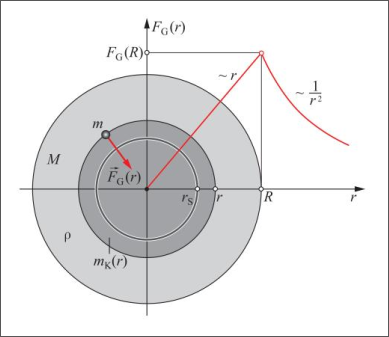
\includegraphics[scale=0.3]{2023_01_01_02_52_53.png}
}[0.25,0.25]

\subsubsection{Gravitational Work}
\, \newline
\large \textcolor{purple}{\( W_{12} = \int_{r_1}^{r_2} G \dfrac{Mm}{r^2}dr = -G\dfrac{Mm}{r}|^{r_2}_{r_1} = GMm\left( \dfrac{1}{r_2} - \dfrac{1}{r_1} \right) \)}\newline
\, \newline
\normalsize

\subsubsection{Gravitational Potential}
\minipg{
\, \newline
\large \textcolor{purple}{\( \phi = \dfrac{E_{pot}}{m} = -\dfrac{GM}{r} \)}\newline
\, \newline
\normalsize Legend: \newline
\begin{itemize}
  \item \(\phi\) = gravitational potential \newline 
    \(\phi = [1\dfrac{1}{kg}]\)
\end{itemize} 
}{
  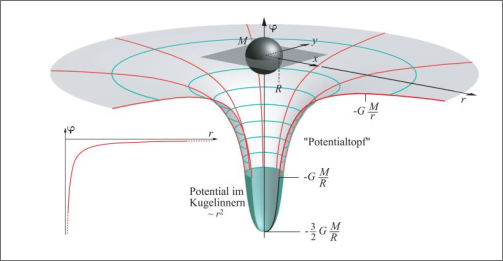
\includegraphics[scale=0.3]{2023_01_01_03_07_59.png}
}[0.20,0.25]

\subsubsection{Gravitational Potential within a homogenous zentral object}
\, \newline
\large \textcolor{purple}{\( F_G = \dfrac{4 \phi G \rho m}{3} * r \)}\newline
\, \newline
\large \textcolor{purple}{\( E_{pot} = -\dfrac{2\phi G \rho m}{3}* r^2 + c' \)}\newline
\, \newline
\large \textcolor{purple}{\( \phi = -\dfrac{2\phi G \rho}{3}* r^2 + c = - \dfrac{GM(r)}{2r} + c\)}\newline
\, \newline
\large \textcolor{orange}{\(
  c = -\frac{GM}{2R} \text{ | } \phi\left(0\right) = \underbrace{-\frac{GM}{R}}_{\text{Potential on ball surface}}\) \newline \(\underbrace{-\frac{GM}{2R}}_{\text{Integrationconstant}}= -\frac{3GM}{2R}
 \)}
\normalsize

\subsection{Context Systems}

\subsubsection{Inertialsystems}
\minipg{
If the newtons laws apply to context system s then it will also apply to context system s' if the new system isn't changed in terms of acceleration. (Centrifugal force for example is considered Acceleration )\newline
\textcolor{orange}{Train with constant velocity is inertial, train with curve -> centrifugal force is not inertial!}
}{
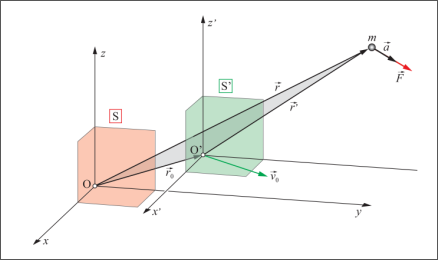
\includegraphics[scale=0.3]{2023_01_01_03_34_46.png}
}[0.23,0.25]

\subsection{Accelerated Context systems}
\subsubsection{InertiaForce}
Within an accelerated context system, the mass of your own body will be used in combination with the acceleration of the context system to append the other acceleration that is applied.
\, \newline
\large \textcolor{purple}{\( \vec{F} = \vec{F} - m\vec{a_0} = \vec{F} + \vec{F_{\text{inertia}}} \text{ => } \vec{F_{\text{inertia}}} = m\vec{a_0} \)}\newline
\, \newline
\normalsize Legend: \newline
\begin{itemize}
\item \(a_0\) = acceleration
\item F = force
\item \(\vec{F_{\text{inertia}}}\) (for example the force of an elevator -> inertia when jumping etc) 
\end{itemize} 
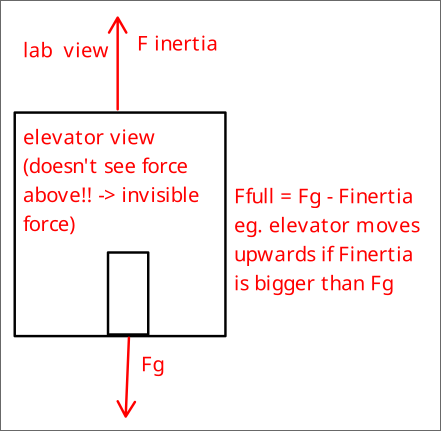
\includegraphics[scale=0.3]{2023_01_01_04_27_36.png}

\subsubsection{Centrifugal Force within context}
\, \newline
\large \textcolor{purple}{\( \vec{F_{ce}} = -m\vec{a_{ce}} = -m * \omega^2 * \vec{r} \)}\newline
\, \newline
\normalsize 
\minipg{
Legend: \newline
\begin{itemize}
  \item \(\vec{F_{ce}}\) = Centrifugal Force == \(\vec{F_z}\)
  \item \(\vec{a_{ce}}\) = Centrifugal acceleration
\item \(\omega\) = angle velocity 
\item r = radius
\item m = mass
\end{itemize} 
}{
  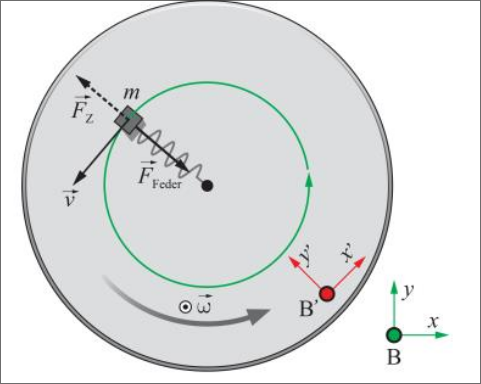
\includegraphics[scale=0.3]{2023_01_01_04_34_43.png}
}[0.25,0.25]

\subsubsection{Coriolis}
\, \newline
\large \textcolor{purple}{\( \vec{a_c} = 2* (\vec{\omega} \text{ x } \vec{v_R}) \)}\newline
\, \newline
\large \textcolor{purple}{\( \vec{F_c} = -m * \vec{a_c} = -m * 2 * (\vec{\omega} \text{ x } \vec{v_R} ) \)}
\, \newline
\normalsize 
\minipg{
Legend: \newline
\begin{itemize}
  \item \(\vec{F_c}\) = coriolis force
  \item \(\vec{a_c}\) = coriolis acceleration
  \item \(\vec{\omega}\) = angle velocity
\item m = mass
\item \(\vec{v_R}\) = angle velocity
\end{itemize} 
}{
  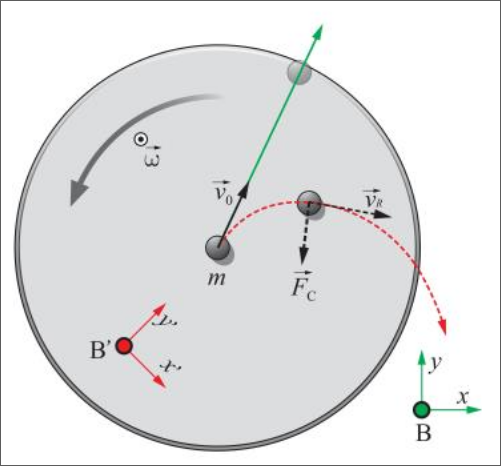
\includegraphics[scale=0.3]{2023_01_01_04_34_50.png}
}[0.25,0.25]

\subsubsection{Lambert}
The applied force, the centrifugal force and the coriolis force will negate each other if the object is in balance!! -> zero vector!
\, \newline
\large \textcolor{purple}{\( \vec{F} + \vec{F_{ce}} + \vec{F_c} = \vec{0} \)}\newline
\, \newline
\normalsize

\subsection{Rotation of rigid bodies}

\subsubsection{Rotation vs Turning}
Rotation is done over a fixed axis -> x,y,z \newline
While turning is done over a fixed point -> see bayblade kekw

\subsubsection{Dynamic Base Rule of Rotation}
\, \newline
\large \textcolor{purple}{\( dM = r * dF_t = r * dm * a_t \)}\newline
\, \newline
\normalsize 
\minipg{
Legend: \newline
\begin{itemize}
\item dM = torque over axis
\item \(d\vec{F}\) = Force
\item dm = mass
\item \(dF_a\) = force over axis
\item \(dF_r\) = force over radius 
\item \(dF_t\) = force over tangent
\end{itemize}
\, \newline
\textcolor{orange}{
In this case we only have a tangential rotation, hence the only axis that matters it the tangential one!!}
}{
  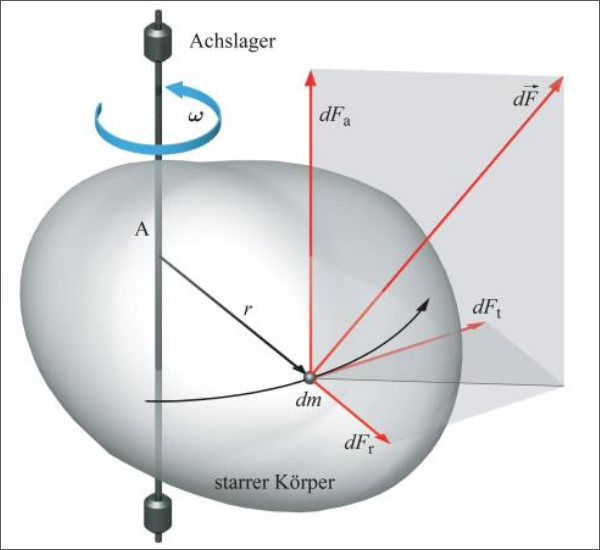
\includegraphics[scale=0.2]{2023_01_01_05_03_12.png}
}[0.25,0.25]

\subsubsection{Moment of Inertia (Trägheitsmoment)}
\, \newline
\large \textcolor{purple}{\( J = \int{r^2 * dm} \)}\newline
\, \newline
\large \textcolor{purple}{\( M = J * a \)}
\, \newline
\normalsize Legend: \newline
\begin{itemize}
\item Moment of Inertia = J
\item \( \alpha \) = angle
\end{itemize}

\subsubsection{Moment of Inertia with different forms}
\begin{itemize}
  \item \textcolor{orange}{Cylinder} \newline
    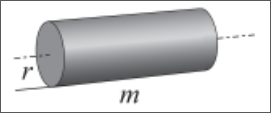
\includegraphics[scale=0.3]{2023_01_01_05_13_04.png}\textcolor{purple}{\( \dfrac{m * r^2}{2} \)}
  \item \textcolor{orange}{Tube} \newline
    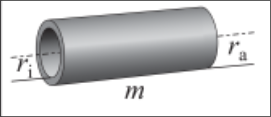
\includegraphics[scale=0.3]{2023_01_01_05_13_11.png}\textcolor{purple}{\( \dfrac{m(r^2_a) + r^2_i}{2} \)}
  \item \textcolor{orange}{Sphere} \newline
    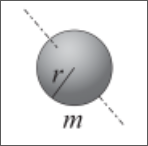
\includegraphics[scale=0.3]{2023_01_01_05_13_13.png}\textcolor{purple}{\( \dfrac{2}{5} m * r^2 \)}
  \item \textcolor{orange}{Block} \newline
    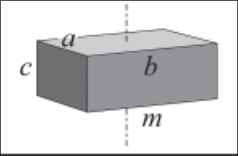
\includegraphics[scale=0.3]{2023_01_01_05_13_16.png}\textcolor{purple}{\( \dfrac{m(a^2 + b^2)}{12} \)}
\end{itemize} 

\subsubsection{Inertia radius}
\, \newline
\large \textcolor{purple}{\( r_0 = \sqrt{\dfrac{J}{M}} \)}\newline
\, \newline
\normalsize Legend: \newline
\begin{itemize}
\item \(r_0\) = inertia radius
\item J = Inertia moment
\item M = torque 
\end{itemize} 

\subsubsection{Moment of Inertia on any axis}
\, \newline
\large \textcolor{purple}{\( J_A = J_x cos^2 \alpha + J_y cos^2 \beta + J_z cos^2 \gamma \)}\newline
\, \newline
\normalsize Legend: \newline
\begin{itemize}
\item The angles are from each axis
\item \(J_A\) = Total moment of inertia
\end{itemize} 

\subsubsection{Steiners Rule}
When you have 2 axes, you can calculate the second inertia moment by adding the mass multiplied with the square of the distance between the 2 axes.\newline
\minipg{
\, \newline
\large \textcolor{purple}{\( J_A = J_s + m * d^2 \)}\newline
\, \newline
\normalsize Legend: \newline
\begin{itemize}
\item \(J_A\) = inertia moment of axis A
\item \(J_S\) = Inertia moment of axis \(A_S\)
\item m = mass
\item d = distance between axes
\end{itemize} 
}{
  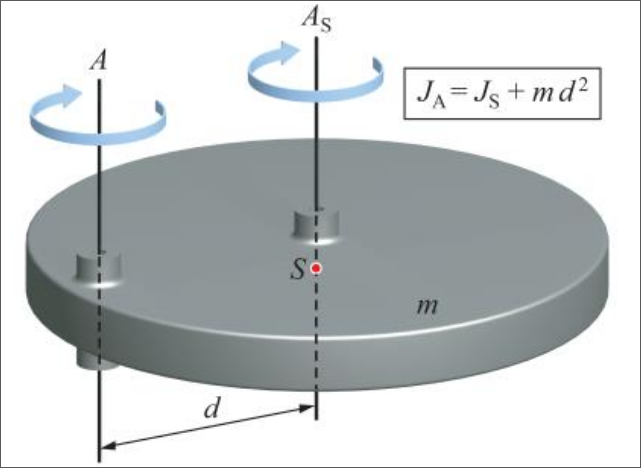
\includegraphics[scale=0.2]{2023_01_01_05_19_52.png}
}[0.25,0.25]

\subsubsection{Work on Rotation}
\, \newline
\large \textcolor{purple}{\( dW = \vec{F}d\vec{s} = F_t ds = F_t * r * d\phi = Md\phi \)}\newline
\, \newline
\normalsize Legend: \newline
\begin{itemize}
\item dW = Work
\item \(\vec{F_t}\) = force of rotation
\item ds = distance 
\item \(\phi\) = angle of rotation (angle between start and end)
\end{itemize} 

\subsubsection{Power of Rotation}
\, \newline
\large \textcolor{purple}{\( P = \dfrac{dW}{dt} = M \dfrac{d\phi}{dt} = M\omega \)}\newline
\, \newline
\normalsize Legend: \newline
\begin{itemize}
\item P = power
\item dW = Work
\item dt = time  
\item M = torque
\item \(\phi\) = angle between start and end 
\item \(\omega\) = angle velocity
\end{itemize} 

\subsubsection{Energies}
\large \textcolor{orange}{Translation-Energy}\newline
\, \newline
\large \textcolor{purple}{\( E_{\text{trans}} = \dfrac{1}{2}mv^2_s \)}\newline
\, \newline
\large \textcolor{orange}{Rotation-Energy}\newline
\, \newline
\large \textcolor{purple}{\( E_{\text{rot}} = \dfrac{1}{2}J_s\omega^2 \)}
\, \newline
\large \textcolor{orange}{Total}\newline
\, \newline
\large \textcolor{purple}{\(E_{\text{tot}} = E_{\text{trans}} +  E_{\text{rot}}\)}
\normalsize

\subsubsection{Turning Impulse}
\, \newline
\large \textcolor{purple}{\( \vec{L} = \vec{r} \text{ x } \vec{p} \)}\newline
\, \newline
\large \textcolor{purple}{\( \vec{L} = \int{d\vec{L}} = \int{\vec{r} \text{ x } \vec{v} * dm} \)}\newline
\, \newline
\normalsize Legend: \newline
\begin{itemize}
  \item \(\vec{L}\) = Turning Impulse
  \item \(\vec{r}\) = radius as vector
  \item \(\vec{v}\) = velocity as vector 
\item dm = mass
\item \(d\vec{p}\) = impulse force = \(\vec{F}\)
\end{itemize} 
\includegraphics[scale=0.2]{2023_01_01_07_14_44.png}

\subsubsection{torque vs Turning impulse}
\, \newline
\large \textcolor{purple}{\( \vec{F} = m * \vec{a} = m * \dfrac{d\vec{v}}{dt}  = \dfrac{d\vec{p}}{dt}\)}\newline
\, \newline
\large \textcolor{purple}{\( \vec{M} = \vec{r} \text{ x } \vec{F} = \dfrac{d}{dt} (\vec{r} \text{ x } \vec{p}) = \dfrac{d}{dt} \vec{L} = \vec{L_2} \)}\newline
\, \newline
\large \textcolor{purple}{\( \dfrac{d\vec{L}}{dt} = 0 \)} within a closed system!!\newline
\, \newline
\normalsize Legend: \newline
\begin{itemize}
  \item \(\vec{L}\) = turning impulse
  \item \(\vec{M}\) = torque
  \item \(\vec{L_2}\) = new turning impulse  
\item dt = time
\end{itemize}
\textcolor{red}{Withing a closed system, the impulse is never lost!!}

\subsubsection{Turning impulse vs angle velocity}
\, \newline
\large \textcolor{purple}{\( M = J\dfrac{d\omega}{dt} = \dfrac{d\vec{L}}{dt} \)}\newline
\, \newline
\large \textcolor{purple}{\( \vec{L} = J \vec{\omega} \)}
\, \newline
\normalsize Legend: \newline
\begin{itemize}
\item M = torque
\item J = Moment of inertia
\item \(\vec{L}\) = Turning impulse 
\item \(\vec{\omega}\) = angle velocity
\item dt = time
\end{itemize} 

\subsection{gyroscope}
\subsubsection{Force free gyroscope}
\, \newline
\large \textcolor{purple}{\( \vec{M} = \vec{0} \) and \( \vec{L} = \text{constant} \)}\newline
\, \newline
\large \textcolor{orange}{When a symmetric gyroscope spins:}
\, \newline
\large \textcolor{purple}{\( \vec{L} = J\vec{\omega} \)}\newline
therefore \(\omega\) and J are also constant!\newline
\, \newline
\normalsize Legend: \newline
\begin{itemize}
  \item \(\vec{M}\) = torque
  \item \(\vec{L}\) = Turning impulse
\item \(\omega\) = angle velocity 
\item J = moment of inertia
\end{itemize} 

\subsubsection{Forces on gyroscope}
\, \newline
\large \textcolor{purple}{\( d\vec{L} = \vec{M}dt \)}\newline
\(\omega dt >> d\phi\) fast rotation!\newline
\, \newline
\normalsize Legend: \newline
\begin{itemize}
  \item \(\vec{L}\) = Turning impulse
  \item \(\vec{M}\) = torque
\item dt = time  
\item \(d\phi\) = angle 
\item \(\omega\) = angle velocity
\end{itemize} 

\subsubsection{Precision gyroscope}
\, \newline
\large \textcolor{purple}{\( \Omega = \dfrac{d\phi}{dt} = \dfrac{1}{L sin(\beta)} * \underset{M}{\dfrac{dL}{dt}} \)}\newline
\, \newline
\normalsize Legend: \newline
\begin{itemize}
\item \(\Omega\) = Precision angle velocit
\item d\(\phi\) = angle between current pos and next pos
\item dt = time  
\item L = Turning impulse
\item dL = second impulse 
\item \(\beta\) = angle between original starting orientation and current orientation
\end{itemize}
\includegraphics[scale=0.2]{2023_01_01_07_32_08.png}

\end{multicols*}
\end{document}

